%%%%%%%%%%%%%%%%%%%%%%%%%%%%%%%%%%%%%%%%%%%%%%%%%%%%%%%%%%%%%%%%%%%%%%%%%%%%%%%%%%%%%%%%%%%%%%%%
%
% CSCI 1430 Written Question Template
%
% This is a LaTeX document. LaTeX is a markup language for producing documents.
% Your task is to answer the questions by filling out this document, then to
% compile this into a PDF document.
%
% TO COMPILE:
% > pdflatex thisfile.tex

% If you do not have LaTeX, your options are:
% - VSCode extension: https://marketplace.visualstudio.com/items?itemName=James-Yu.latex-workshop
% - Online Tool: https://www.overleaf.com/ - most LaTeX packages are pre-installed here (e.g., \usepackage{}).
% - Personal laptops (all common OS): http://www.latex-project.org/get/ 
%
% If you need help with LaTeX, please come to office hours.
% Or, there is plenty of help online:
% https://en.wikibooks.org/wiki/LaTeX
%
% Good luck!
% The CSCI 1430 staff
%
%%%%%%%%%%%%%%%%%%%%%%%%%%%%%%%%%%%%%%%%%%%%%%%%%%%%%%%%%%%%%%%%%%%%%%%%%%%%%%%%%%%%%%%%%%%%%%%%
%
% How to include two graphics on the same line:
% 
% \includegraphics[width=0.49\linewidth]{yourgraphic1.png}
% \includegraphics[width=0.49\linewidth]{yourgraphic2.png}
%
% How to include equations:
%
% \begin{equation}
% y = mx+c
% \end{equation}
% 
%%%%%%%%%%%%%%%%%%%%%%%%%%%%%%%%%%%%%%%%%%%%%%%%%%%%%%%%%%%%%%%%%%%%%%%%%%%%%%%%%%%%%%%%%%%%%%%%

\documentclass[10pt,twocolumn,letterpaper]{article}
 
\usepackage{cvpr}
\usepackage{times}
\usepackage{epsfig}
\usepackage{graphicx}
\usepackage{amsmath}
\usepackage{amssymb}
\usepackage{booktabs}
\usepackage{microtype}
% From https://ctan.org/pkg/matlab-prettifier
\usepackage[numbered,framed]{matlab-prettifier}

\frenchspacing

% Include other packages here, before hyperref.

% If you comment hyperref and then uncomment it, you should delete
% egpaper.aux before re-running latex.  (Or just hit 'q' on the first latex
% run, let it finish, and you should be clear).
\usepackage[pagebackref=true,breaklinks=true,letterpaper=true,colorlinks,bookmarks=false]{hyperref}

\cvprfinalcopy
\def\cvprPaperID{****}
\def\httilde{\mbox{\tt\raisebox{-.5ex}{\symbol{126}}}}
\ifcvprfinal\pagestyle{empty}\fi

\begin{document}

%%%%%%%%% TITLE
\title{CSCI 1430 Final Project Report:\\Is That Santa}

% Make this document not anonymous
\author{
    \emph{Team name}: IS SANTA REAL\\
    \emph{TA name:} David Grossman
    Brown University\\
}

\maketitle
%\thispagestyle{empty}

%%%%%%%%% ABSTRACT
\begin{abstract}
This paper explores the age old question: "is that person I saw santa claus or not". 
We develop a model using two different techinques and compare the results. In creating these models, we explore and utilize various techniques to combat overfitting, while increasing our accuracy and maximing the metrics chosen. 
\end{abstract}


%%%%%%%%% BODY TEXT
\section{Introduction}

Generally we think of santa as the western interpretation. This presents some representation issues as santa is depicted in many different ways across many different cultures. The goal of this project is to create a model that can classify santa considering the many different cultural interpretations of santa. Some of the challenges presented are data collection, measuring accuracy of model, and the model itself - more specifically its architecture.


\section{Related Work}
We didn't reference too many models, however we did use a lot of external software and libraries. The following is a list:
\begin{itemize}
    \item \href{https://pypi.org/project/python-dotenv/}{dotenv}: environment variables are managed using this package.

    \item \href{https://cmd2.readthedocs.io/en/stable/}{cmd2}: cli interface package for python. Made it easier to run the redundant python scripts when collecting data
    
    \item \href{https://pypi.org/project/opencv-python/}{cv2}: bunch of different uses, but one unique one is for facial recognition command in cli. That model was found online after searching google
    
    \item \href{https://www.tensorflow.org/api_docs/python/tf}{tensorflow}: this is what we actually used to build the model 
    \item \href{https://www.kaggle.com/docs/api}{kaggle api}: this is how we get the dataset locally (before using gcp). Requires an account but is every easy to use and free
    \item \href{https://cloud.google.com/python/docs/reference}{gcp api}: this is how we interact with gcp. Requires an account and project. More complicated to set up than kaggle.
    \item \href{https://github.com/chuanqi305/MobileNet-SSD/blob/master/mobilenet_iter_73000.caffemodel}{pretrained model} for facial recognition
    
    
    
\end{itemize}

\section{Method}
Our goal for this classification project is to be able to classify the testing dataset at 90\% accuracy. We are also looking to maximize recall and f1 score, both of which we discuss in further detail below. 
We thought this was a fair goal because the images we collected for our dataset seemed to be very different 
from the negative set, making it easier to classify. We will discuss how that data was collected as well as how the model was built and other factors.
\subsection{Dataset}
We created our own dataset of santa positive and negative images for this assignment. Using the google search query api, we requested 
~5000 images from Google. Afterwards, we used a pretrained model found online trained on ImageNet for facial detection. With this, we removed 
images that contained 0 faces or more than 1 face. We removed duplicates and manually removed images that were not appropriate or did not fit within the 
guidelines of what we defined as Santa. We ended up with two versions of the dataset. The \href{https://www.kaggle.com/datasets/ianmaloney/santa-images}{first version} was larger and balanced (1420 images), but contained more noisey images. The 
\href{https://www.kaggle.com/datasets/ianmaloney/updated-santa}{second version} was smaller and imbalanced (793 images), but had no noisey images. 

The following are a few examples of queries used to compile the positive and negative images:
\begin{itemize}
    \item santa claus inpersonator
    \item white bearded man
    \item person
    \item person portrait
\end{itemize}

There is a more exhaustive list of searches in the readme of the code portion. 

\subsection{Model}


This model consisted of 5 convolutional layers, each of increasing filter size.
\begin{enumerate}
    \item 3 filters, kernel size 3
    \item 3 filters, kernel size 4 
    \item 30 filters, kernel size 5 
    \item 100 filters, kernel size 4 
    \item 250 filters, kernel size 4 
    \item flatten 
    \item dense layer 
\end{enumerate}
\begin{figure}[h]
    \centering
    
\includegraphics[width=\linewidth]{img/santa.jpg}
    \caption{Non-Transfer Model.}
    \label{fig:result1}
\end{figure}

We used a leaky relu activation function for the convolutional layers and a sigmoid activation function for the dense layer.
These parameters were derived from tweaking the model over time. One issue presented in developing this model was logging. 
In earlier stages of the model, logging was not robust and did not capture all data necessary to pain the full picture. 


\subsection{Transfer Model}
This model consisted of 8 layers. 
\begin{enumerate}
    \item pretrained head using Google's inception v3
    \item conolutional layer with 3 filters and kernel size of 4
    \item upsampling by 10
    \item conolutional layer with 3 filters and kernel size of 4
    \item convolutional layer with 5 filters and kernel size of 5 
    \item convolutional layer with 8 filters and kernel size of 5 
    \item spatial dropout
    \item upsampling by 4 
    \item convolutional layer with 8 filters and kernel size of 5 
    \item spatial dropout 
    \item convolutional layer with 20 filters and kernel size of 4 
    \item flatten 
    \item dropout 
    \item dense layer
\end{enumerate}
Just like the original model, we used leaky relu for our convolutional layers and sigmoid for our dense layers. 
We also included regularization at eacfh layer.
\subsection{Hyperparameters}
\begin{lstlisting}[style=Matlab-editor]
    min_learning_rate = 1e-05
    max_learning_rate = 0.001
    num_epochs = 50
    batch_size = 15
    image_size = 256
    num_classes = 2
    validation_split = 0.18
    leaky_relu_alpha = 0.3
    dropout = 0.7
    gamma = 3.0
    momentum = 0.8
    patience = 5
    test_batch_size = 6
\end{lstlisting}



\subsection{Techniques}
We tried four different things in order to improve accuracy:
\begin{itemize}
    \item \textbf{Learning Rate Scheduler} - we opted to use an increasing learning rate proportionate to the number of epochs used. This function was a logistic smoothing function that increased over time. The function didn't smooth and we think it may have affected results negatively.
    \begin{figure}[h]
        \centering
        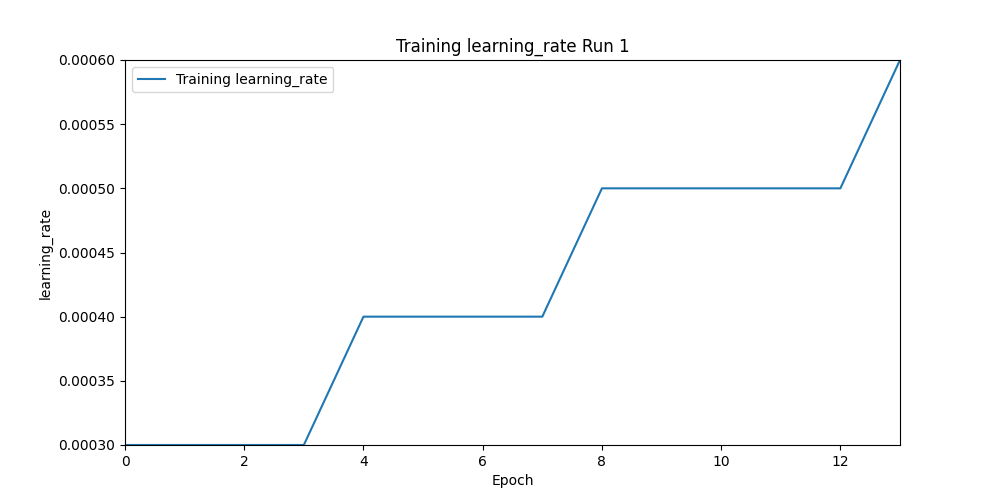
\includegraphics[width=\linewidth]{img/training_learning_rate_run_1.png}
        \caption{Learning Rate}
        \label{fig:result1}
    \end{figure}
    
    \item \textbf{Early Stopping} - If the loss remained stagnant or increased over a number of epochs, training would end. This saved us time in that if a model were becoming grossly overfit, we would just stop training immediately. We call this value our patience value. We began with a patience value of 8, but decreased it to 3 overtime.
    \item \textbf{Data Augmentation} - We tried to augment the data with some different techniques such as brightness, vertical and horizontal shifting, shear, and rotation. 
    \item \textbf{Samplewise Center} - Each individual image is independently normalized. Given that our images are different both due to their own general appearances and the data augmentation process, we felt it would make sense to normalize them according to their own information rather than a mean of images (which could be sensitive to outliers).
\end{itemize}


\section{Results}
Our results were mixed because although we didn't make our projected goal of 90\% accuracy, we were able to 
produce a model that was able to predict whether santa is present or not at 70\% accuracy. There were a few things that could have been improved in this experiment. 

\begin{figure}[h]
    \centering
    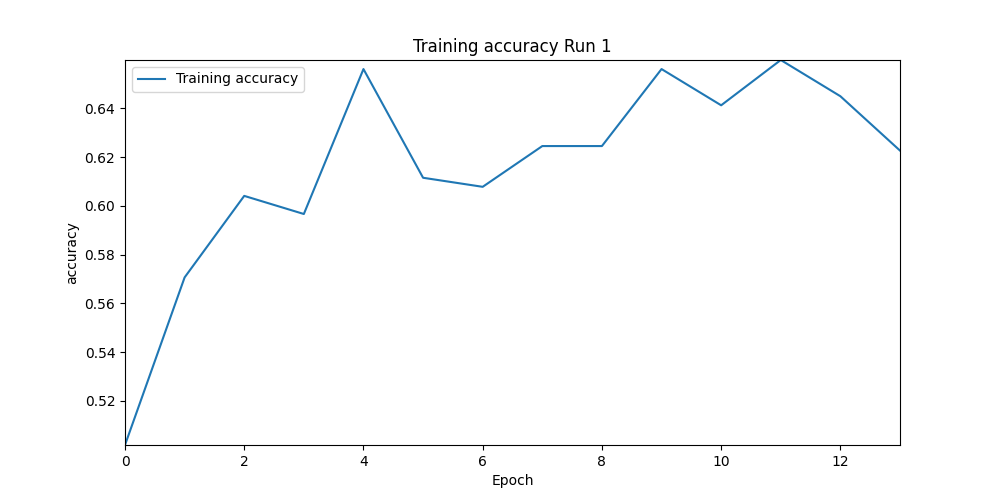
\includegraphics[width=0.30\linewidth]{img/training_accuracy_run_1.png}
    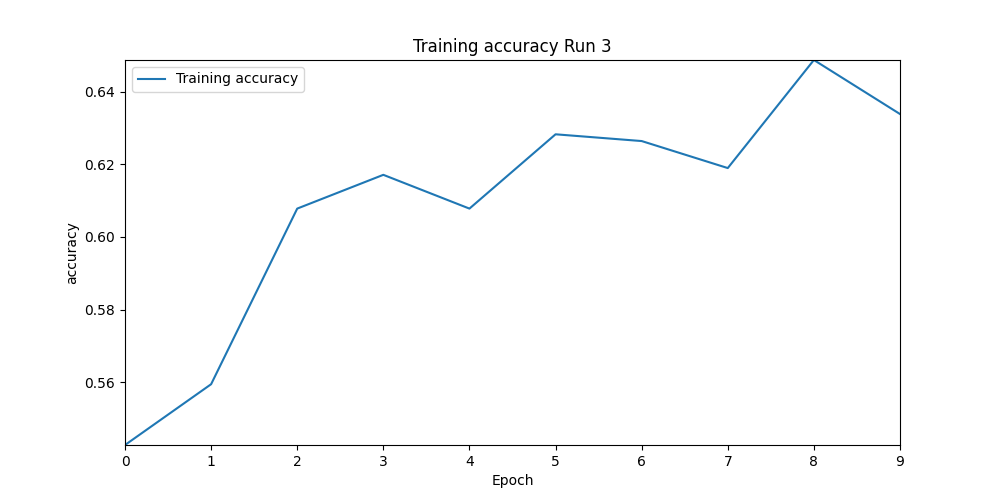
\includegraphics[width=0.30\linewidth]{img/training_accuracy_run_3.png}
    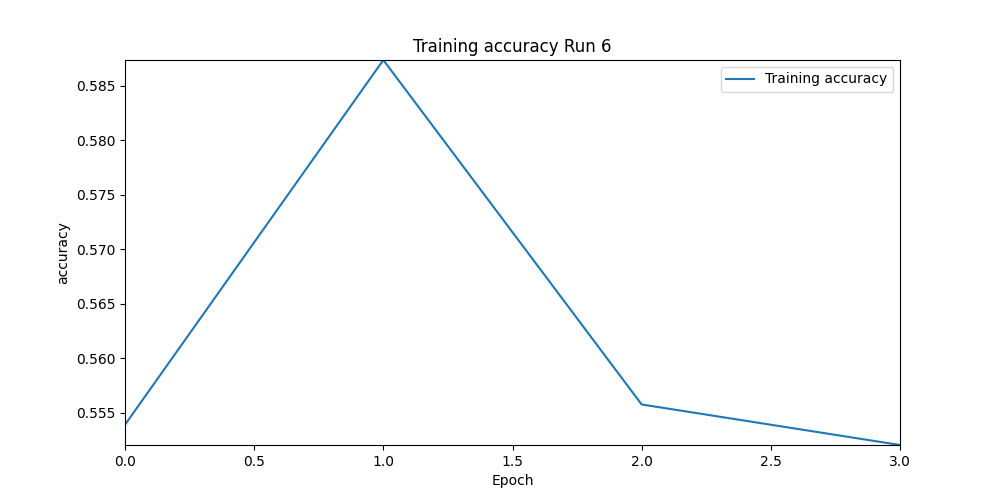
\includegraphics[width=0.30\linewidth]{img/training_accuracy_run_6.png}
    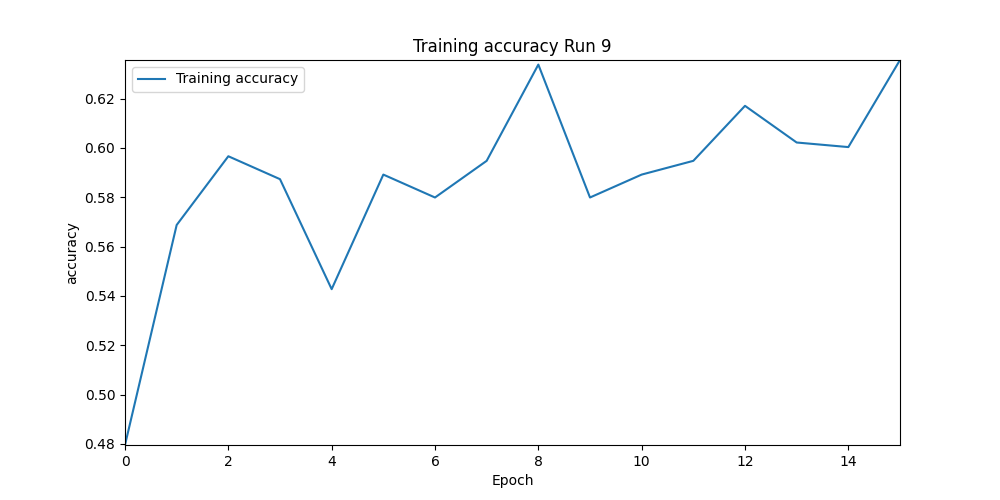
\includegraphics[width=0.30\linewidth]{img/training_accuracy_run_9.png}
    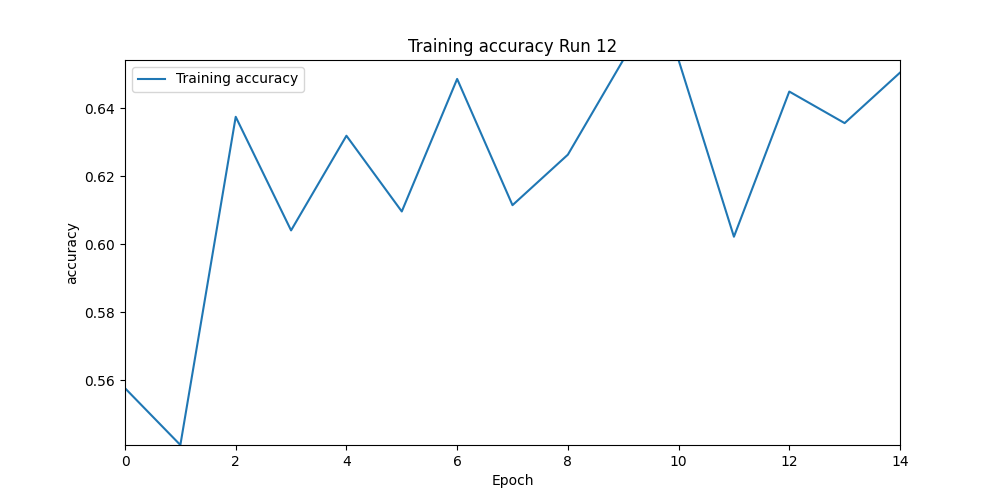
\includegraphics[width=0.30\linewidth]{img/training_accuracy_run_12.png}
    \caption{Accuracy over runs}
    \label{fig:result2}
\end{figure}

One thing that became clear was misclassification was in part due to some of the data augmentation. We used a very large range for brightness shifts which caused some images to come out near black. 
This images seemed to be very difficult for the model to classify and contributed heavily to a lot of the misclassifications. As seen in the following figure, all misclassified examples are dark images.
\begin{figure}[h]
    \centering
    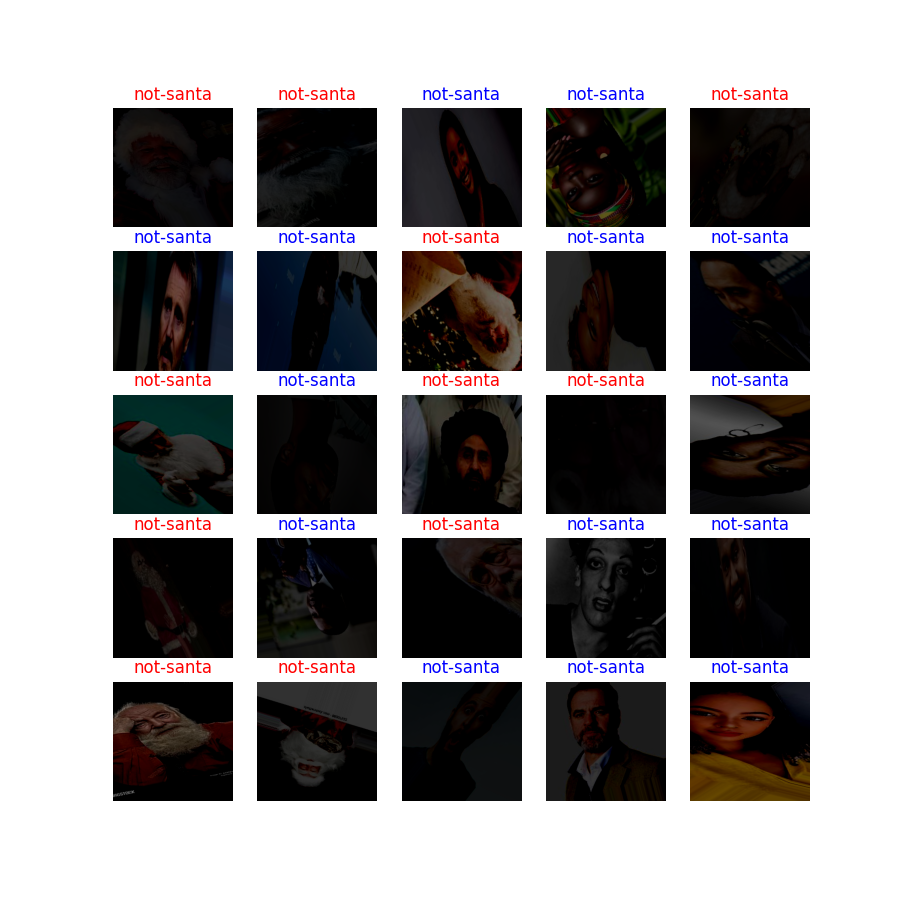
\includegraphics[width=0.70\linewidth]{img/imageData-4.png}
    \caption{Mislabeled/ Hardest Classifications}
    \label{fig:result2}
\end{figure}

%-------------------------------------------------------------------------
\subsection{Technical Discussion}

One of the biggest trade offs in designing this project was using the smaller dataset. 
We originally had a dataset of 1420 images but decided to remove what was considered noise/ did not fit what we were trying to model. 
This included any images that were not santa, images that were not human, images that were full body images of santa, and female santa claus. 
The reason we did not include images of full body santas and female is because these images either included a lot of noise in them or they were inappropriate. 
We focused on images of men with beards when training this model to make up for the lack of diversity. 
Using the smaller dataset meant we were using an imbalanced dataset which presented its own issues.



The use of the imbalanced dataset presented a few challenges, especially considering this is a binary classification problem. 
With an imbalanced dataset, results are skewed in favor of the majority class. 
In our case, this was guessing not santa when presented with a difficult sample. 
We did three things to help combat this issue. First, we added class weights to the training model in order to balance the difference. 
The amount of images weren't completely different so so santa images ended up being a little more important than not santa. 
We knew it was favoring the not santa prediction because we saw many false negatives in the early stages of the model. 

\begin{figure}[h]
    \centering
    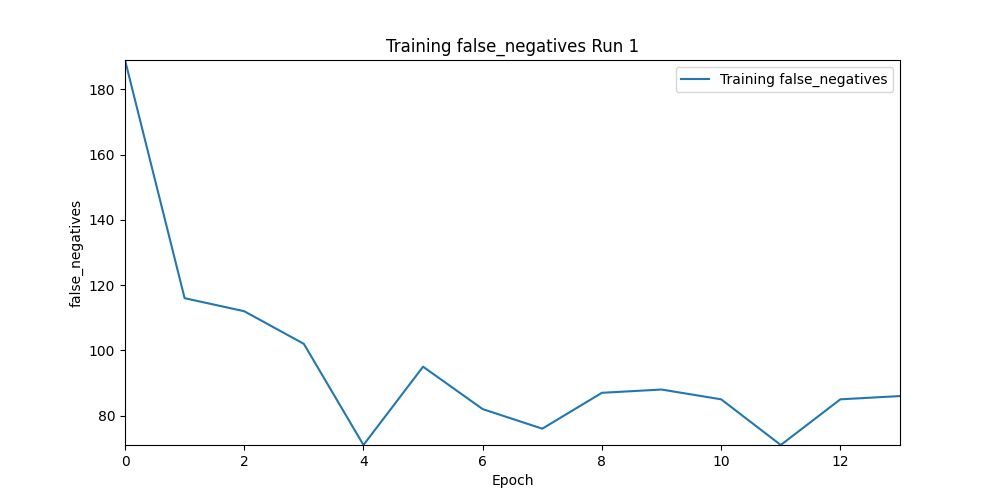
\includegraphics[width=0.30\linewidth]{img/training_false_negatives_run_1.png}
    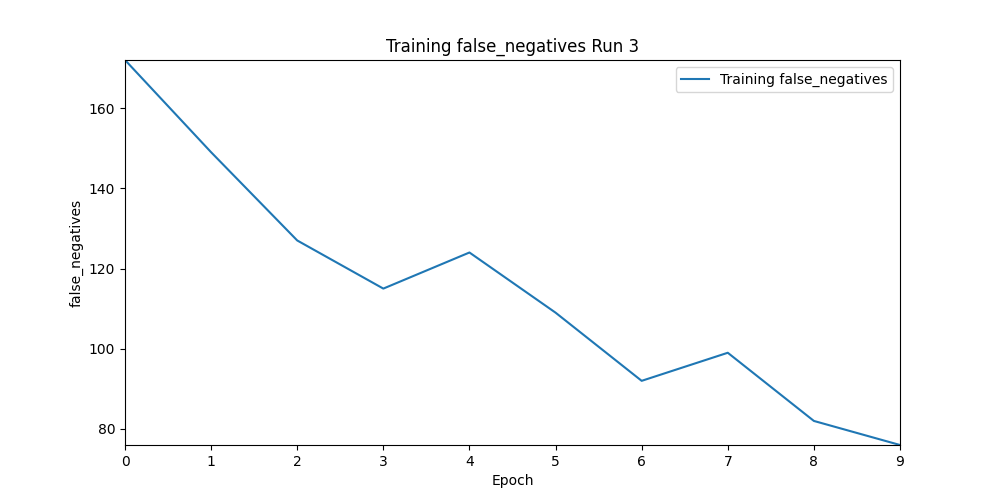
\includegraphics[width=0.30\linewidth]{img/training_false_negatives_run_3.png}
    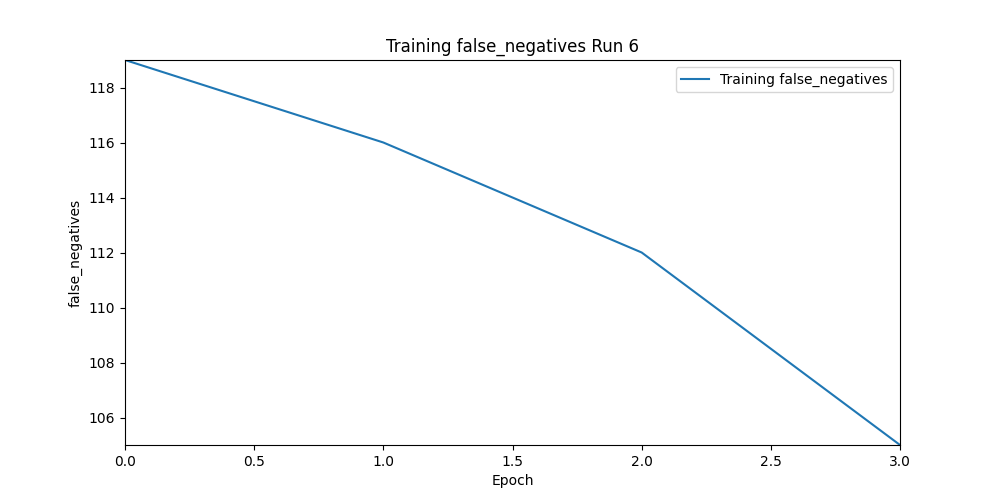
\includegraphics[width=0.30\linewidth]{img/training_false_negatives_run_6.png}
    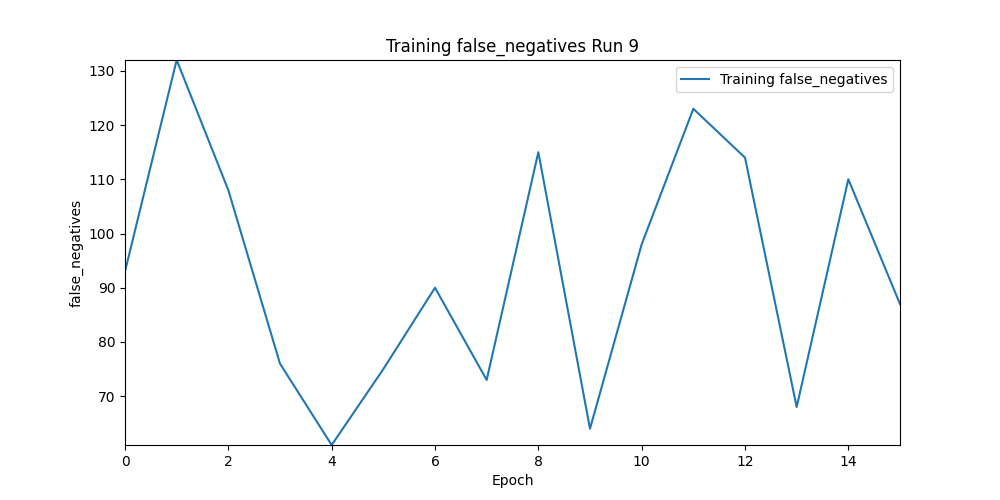
\includegraphics[width=0.30\linewidth]{img/training_false_negatives_run_9.png}
    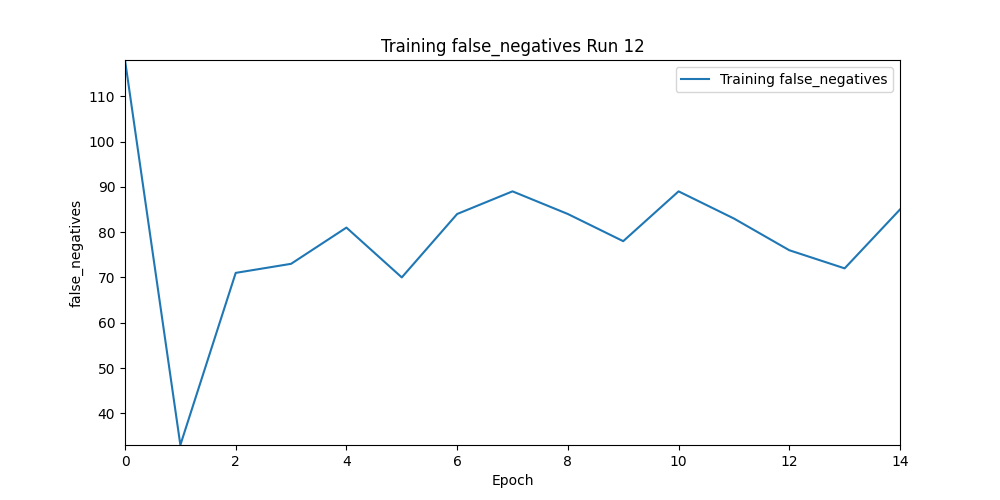
\includegraphics[width=0.30\linewidth]{img/training_false_negatives_run_12.png}
    \caption{False Negatives over runs}
    \label{fig:result2}
\end{figure}

We used the number of false negatives over each iteration of the model as an indicator of whether we improved the imbalance issue or not. 
The final thing we did was adjust the loss function. Other metrics used to help evaluate were accuracy, recall, and f1 score. As mentioned before, accuracy wasn't as reliable 
given our imbalanced dataset. 



We used recall as it places more emphasis on positive indentifications rather than overall accuracy. 
Correct Positive predictions were rarer. F1 score was helpful in keeping recall in check because we noticed at times, 
higher recall would correspond to a higher likelihood of overfitting. 

\begin{figure}[h]
    \centering
    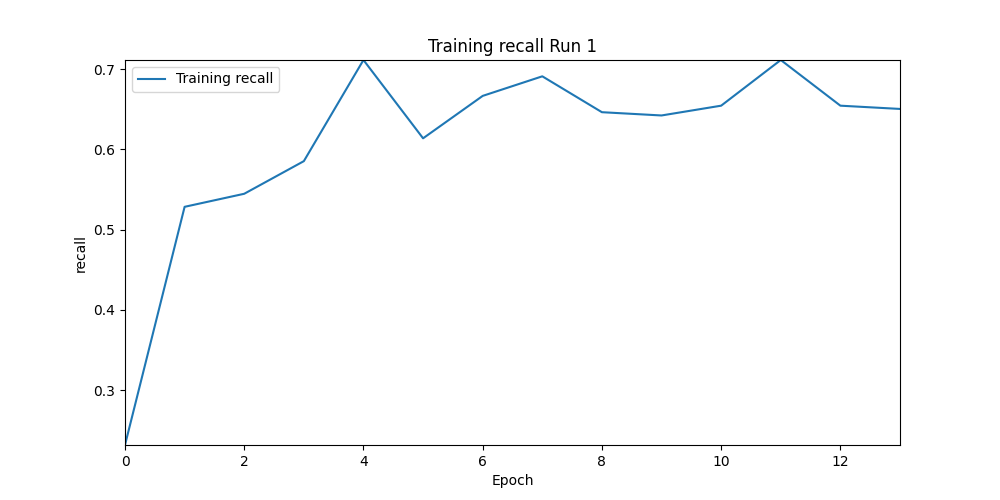
\includegraphics[width=0.30\linewidth]{img/training_recall_run_1.png}
    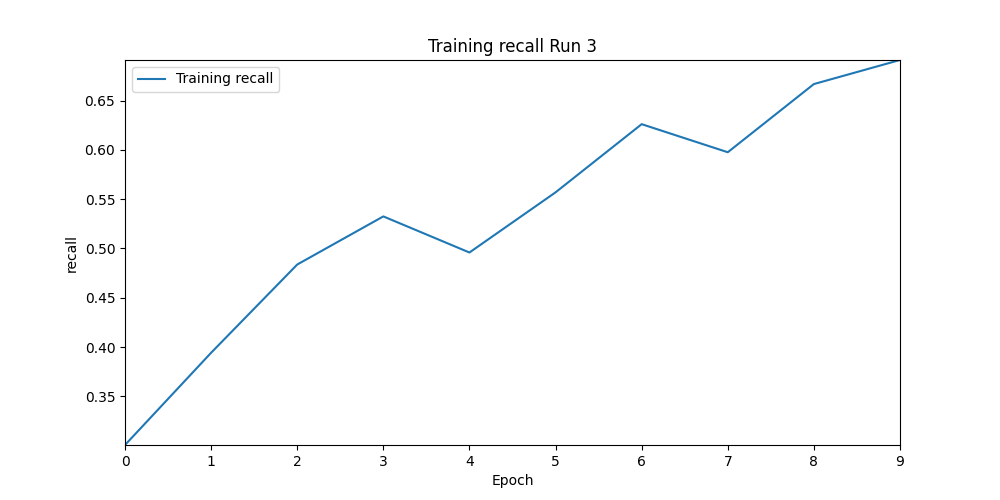
\includegraphics[width=0.30\linewidth]{img/training_recall_run_3.png}
    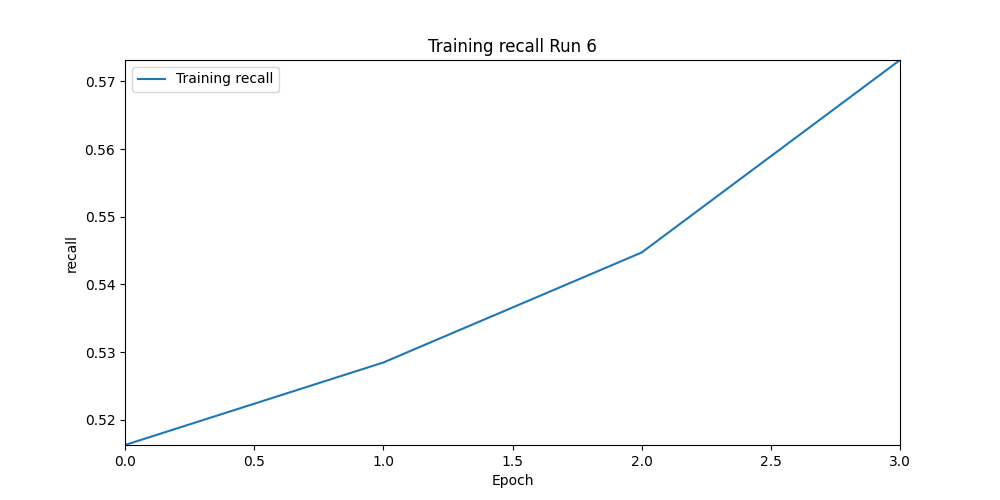
\includegraphics[width=0.30\linewidth]{img/training_recall_run_6.png}
    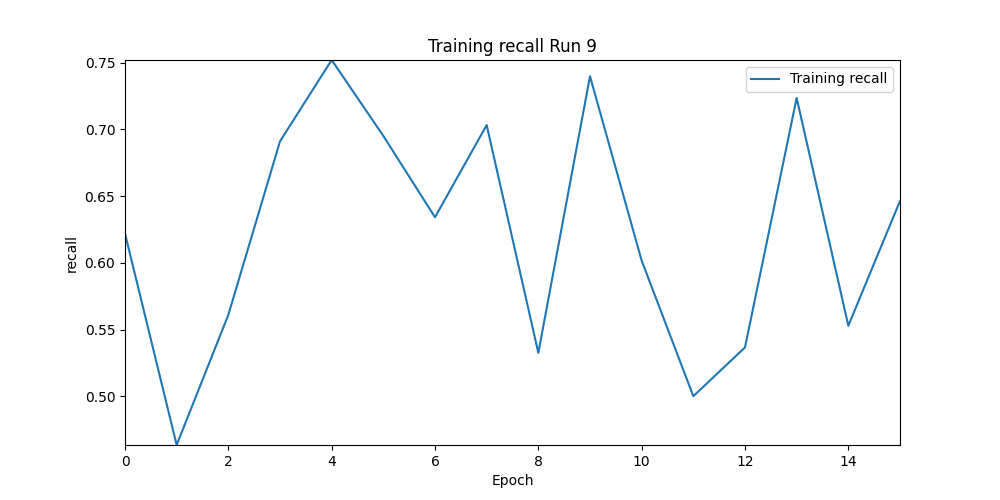
\includegraphics[width=0.30\linewidth]{img/training_recall_run_9.png}
    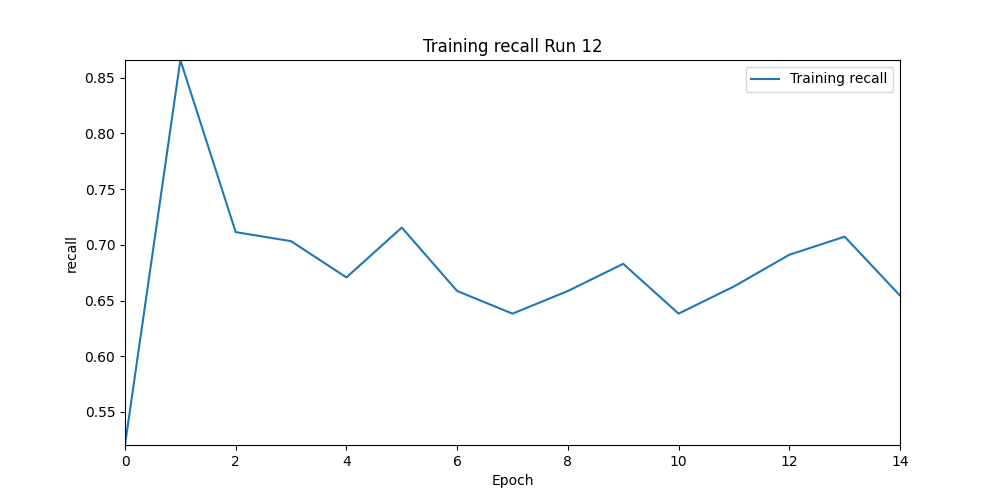
\includegraphics[width=0.30\linewidth]{img/training_recall_run_12.png}
    \caption{Recall over runs}
    \label{fig:result2}
\end{figure}

\begin{figure}[h]
    \centering
    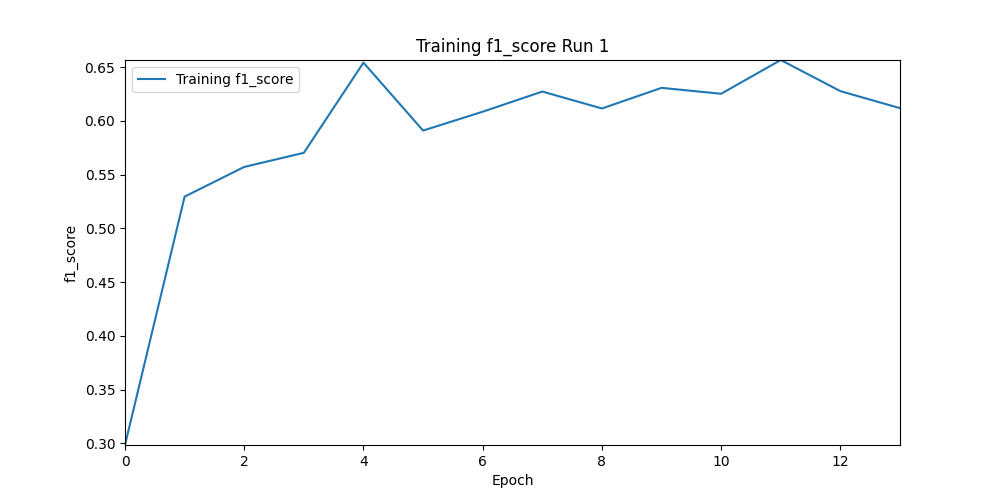
\includegraphics[width=0.30\linewidth]{img/training_f1_score_run_1.png}
    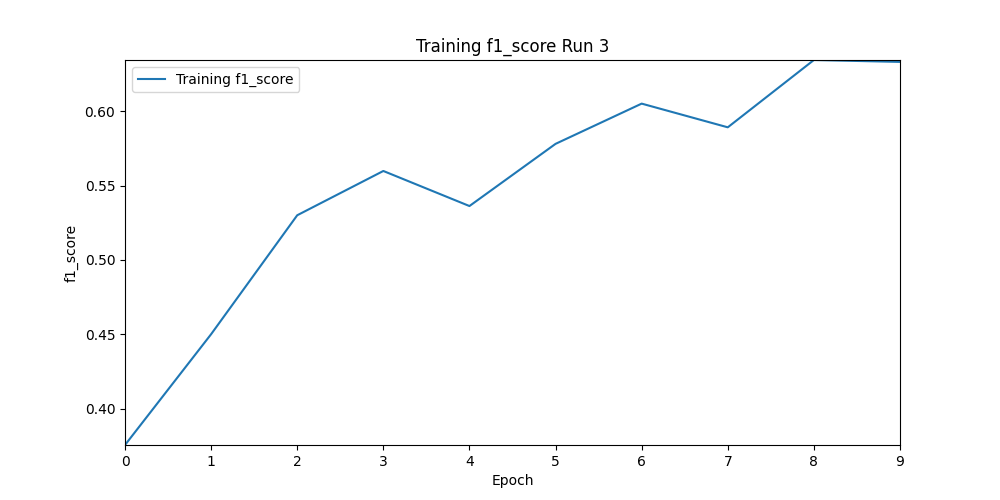
\includegraphics[width=0.30\linewidth]{img/training_f1_score_run_3.png}
    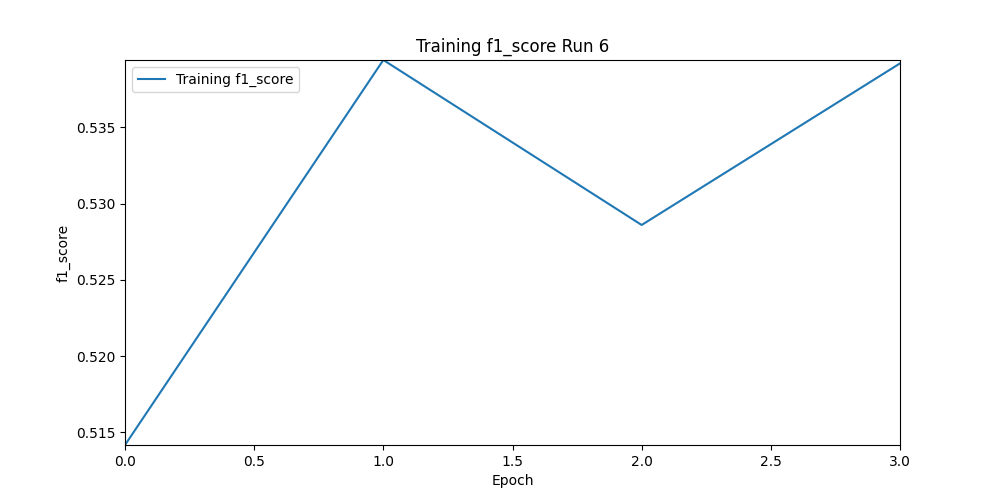
\includegraphics[width=0.30\linewidth]{img/training_f1_score_run_6.png}
    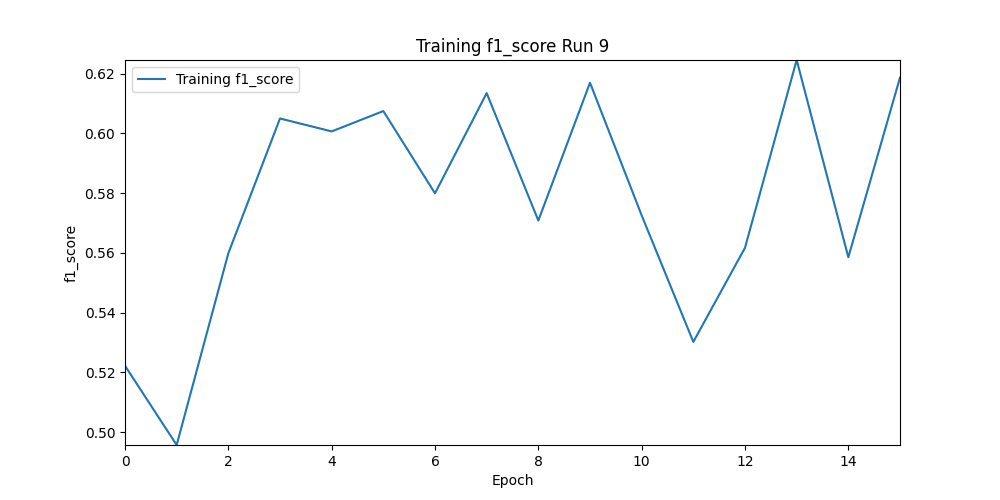
\includegraphics[width=0.30\linewidth]{img/training_f1_score_run_9.png}
    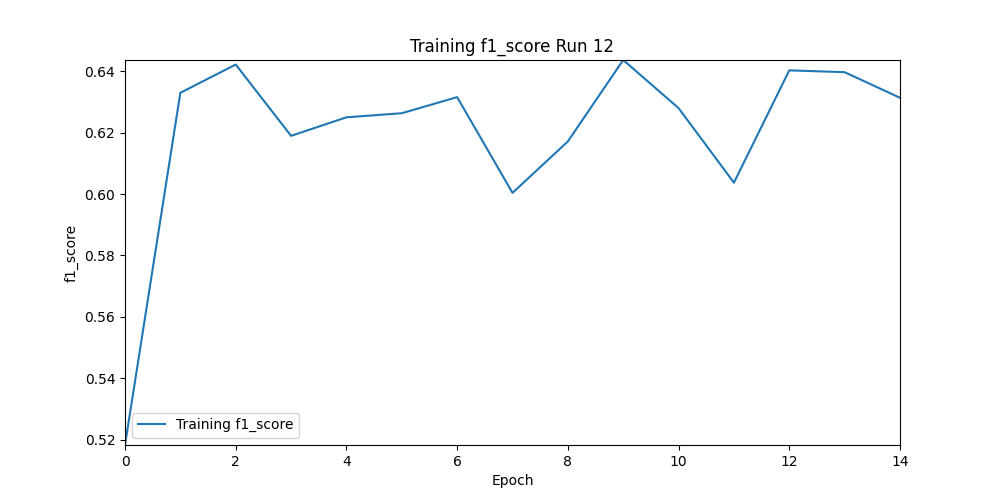
\includegraphics[width=0.30\linewidth]{img/training_f1_score_run_12.png}
    \caption{F1 Score over runs}
    \label{fig:result2}
\end{figure}

We opted to use binary focal crossentropy loss because it allowed us to weight harder 
classifications with more value. Easy classifications would have less weight because we more examples of one class and the model would most likely 
guess this class in the event it didnt't know.

One final note is the learning rate scheduler may have worked against the model. Since the smoothing was to occur over the course of all 50 epochs, the model may not 
actually achieve the maximum learning rate due to early stopping. Early stopping was essential to monitoring the loss of the model, yet if we stopped at epoch 10, we would 
miss 40 epochs of an increasing learning rate. At this point of stopping the model, the learning rate may have been too small to have learned anything.



%-------------------------------------------------------------------------
\subsection{Socially-responsible Computing Discussion via Proposal Swap}

We respond to the following concerns:
\begin{enumerate}
    \item \textbf{App saving concern}\newline We never intended on saving the image. 
    The model is static in that we are not collecting any more information to train on. Further, given the fact 
    that our accuracy isn't over 95\%, we wouldn't trust labeling when adding to a new dataset. Someone would be 
    required to go and double check the classification. 
    \item \textbf{Data collection concern}\newline Using the robots.txt could potentially lead to copyright infringement 
    issues. We ultimately chose not to retrieve our images by these means because it was more difficult than anticipated. 
    Also, it produced very poor quality images that were not good for usage. Instead we ended up using the google search 
    api as mentioned in the data collection section. It was much cheaper than we intially had budgeted for and it provided 
    higher quality images in a more consistent format which made it easier for further processing. Using the api was free 
    for the first 100 requests per day and then a fraction of a penny for each request afterward. We made 883 requests at a 
    total cost of \$2.21.
    \item \textbf{Avoiding bias with santa representation}\newline This is a reasonable concern and to get around this, we used different 
    queries to increase the amount of diverse representations of santa. For example, we looked up "black santa" to find more african 
    american depictions of santa. Afterwards, we hand picked images to has diverse a dataset as we could given the subject matter. One 
    thing we noticed as we continued with this process, however, is that the images got worse in terms of representations. These images 
    were either offensive or what you wouldn't want to train a model on. This is why our dataset is so small, as we had to remove a lot of 
    images collected. 
\end{enumerate}


%------------------------------------------------------------------------
\section{Conclusion}
This project addresses the serious concern of representation in machine learning, the difficulties that arise when doing so, and the trade offs that 
take place when creating diverse models. Developing a dataset proved to be more challenging than anticpated and this decision affected the trajectory of 
the rest of the model. More emphasis needed to be placed on normalization and balancing, two concerns whose influence is seen on every part of the model. 
Although the model was not close to the accuracy goal, this project presented an incredible learning opportunity, for both developing an ml pipeline using external 
tools and custom logging as well as the various techniques used to increase the accuracy of models all while combating overfitting.


{\small
\bibliographystyle{plain}
\bibliography{ProjectFinal_ProjectReportTemplate}
}

\section*{Appendix}

\subsection*{Team contributions}

There was one member.

\end{document}
